%==========================================================================
% Exemplo de artigo cientifico UNESC
%
% v0.0 versão em 20/09/2023 por Marlon Oliveira
% v1.0 versão em 25/06/2025 por Marlon Oliveira


%==========================================================================

%==========================================================================
% Pacotes utilizados pela UNESC - não delete as linhas abaixo
%==========================================================================
\documentclass{UNESC}
\usepackage[T1]{fontenc}
\usepackage[utf8]{inputenc}%\usepackage[latin1]{inputenc}
\renewcommand{\rmdefault}{phv} % Arial
\renewcommand{\sfdefault}{phv} % Arial
\usepackage[brazilian]{babel}
\usepackage{graphicx}
%\usepackage{subfigure}
\usepackage{hyperref}
\usepackage{quoting}
\usepackage[labelsep=none]{caption}
\DeclareCaptionLabelFormat{figuracomtraco}{#1~#2 -}
\captionsetup[figure]{labelformat=figuracomtraco, labelsep=space}
\captionsetup[table]{labelformat=simple, labelsep=space, textformat=simple}
\DeclareCaptionLabelFormat{tabelacomtraco}{#1~#2 -}
\captionsetup[table]{labelformat=tabelacomtraco}
\captionsetup{labelsep=none}
%\renewcommand{\thefigure}{\arabic{figure} - }
\usepackage{enumitem}
\usepackage{float}
\usepackage{comment}
\usepackage[hang,flushmargin]{footmisc}
\usepackage{array}

\hypersetup{
  setpagesize  = false,
  colorlinks   = true,    % Colours links instead of ugly boxes
  urlcolor     = blue,    % Colour for external hyperlinks
  linkcolor    = black,   % Colour of internal links
  citecolor    = black    % Colour of citations
}
\urlstyle{same}
\usepackage{setspace}

\usepackage[alf,recuo=0.0cm,abnt-emphasize=bf]{abntex2cite} 

%\captionsetup[figure]{justification=raggedright}


%==========================================================================
% Dados do artigo: título, autores e filiação
%==========================================================================
\title{REGISTRO DIGITAL ANIMAL: DIGITALIZANDO A IDENTIFICAÇÃO E CONTROLE DE VACINAÇÃO DE ANIMAIS DE ESTIMAÇÃO}
\author
{
   Gabriel Goulart de Souza\footnote{Curso de Ciência da Computação, Universidade do Extremo Sul Catarinense (Unesc), Criciúma - Santa Catarina - Brasil. gabriel.gsouzza6@unesc.net},
   Diorgines Mattos Machado\footnote{Coorientador(a), Curso de Ciência da Computação, Universidade do Extremo Sul Catarinense (Unesc), Criciúma - Santa Catarina - Brasil. diorginesmattos@unesc.net},
   Allan Farias Favaro\footnote{Orientador(a), Curso de Ciência da Computação, Universidade do Extremo Sul Catarinense (Unesc), Criciúma - Santa Catarina - Brasil. allanfavaro@gmail.com}
}
%==========================================================================
% Início do texto do artigo
%==========================================================================
\begin{document}

\onehalfspacing

\maketitle
%\thispagestyle{fancy}
%\vspace{6pt}

%% Remover comentario apenas para TCC Final
\begin{comment}
\noindent
\textbf{Resumo:} Deve ter uma sequência de frases concisas e objetivas em parágrafo único, sem enumeração de tópicos, de 100 a 250 palavras, seguido, logo abaixo, das palavras representativas do conteúdo do trabalho, isto é, palavras-chave e/ou descritores, conforme a \citeonline{ABNT2021}.

\vspace{0.5em}
\noindent
\textbf{Palavras-chave:} Elemento obrigatório. Devem ser separadas entre si por ponto e vírgula e finalizadas por ponto, com as iniciais em letra minúscula, com exceção dos substantivos próprios e nomes científicos. 

\vspace{1.0em}
\noindent
\textbf{ABSTRACT:} Tradução do resumo em língua vernácula para outro idioma de propagação internacional (em inglês ABSTRACT, em francês RESUMÉ, em espanhol RESUMEN).

\vspace{0.5em}
\noindent
\textbf{Keywords:} keyword 1; keyword 2; keyword 3.

\end{comment}

\section{INTRODUÇÃO}

A relação entre humanos e animais de estimação apresenta mudanças significativas nas últimas décadas, consolidando o conceito de família multiespécie, no qual o animal ocupa uma posição relevante no núcleo familiar \cite{BOLSON2022}. A valorização desse vínculo amplia a demanda por cuidados contínuos com a saúde e o bem-estar animal, ao mesmo tempo em que incentiva o desenvolvimento de soluções tecnológicas voltadas ao acompanhamento clínico e à organização das informações relacionadas aos pets. A presença dos animais nesse contexto reforça a necessidade de mecanismos que assegurem o controle adequado das condições de saúde \cite{MORAES2024}.

O controle das informações da saúde animal ainda ocorre, em muitos casos, por meio de registros físicos, os quais apresentam limitações relacionadas à conservação, ao acesso e à atualização dos dados. A utilização de cadernetas em papel favorece perdas, danos e dificuldades na consulta do histórico vacinal, especialmente em situações que exigem comprovação imediata. A dependência desse formato compromete a continuidade do acompanhamento e limita a disponibilidade das informações em diferentes contextos de uso \cite{BOLSON2022}. A digitalização de registros surge como alternativa para reduzir tais limitações, permitindo o armazenamento estruturado e o acesso facilitado aos dados de saúde. A adoção de soluções digitais amplia a disponibilidade das informações, possibilita atualização em tempo adequado e contribui para a organização do histórico clínico dos animais. A utilização de dispositivos móveis nesse processo favorece o acesso em diferentes ambientes, alinhando-se às práticas contemporâneas de gestão de dados em saúde \cite{VIEIRA2020}.

A aplicação de tecnologias já consolidadas em contextos humanos, como o registro digital de vacinação, evidencia benefícios relacionados à acessibilidade e à organização das informações. A adaptação dessa abordagem ao contexto da saúde animal permite ampliar o controle sobre os dados vacinais e de identificação, contribuindo para a redução da dependência de documentos físicos. A implementação de soluções digitais nesse cenário favorece a integração entre tecnologia e cuidado animal \cite{MARTINS2024}.

Diante disto, a proposta deste estudo consiste no desenvolvimento de uma aplicação multiplataforma voltada ao registro digital de vacinação e à identificação animal. A solução busca estruturar o armazenamento das informações, facilitar o acesso aos dados e reduzir limitações associadas ao uso de registros físicos. A construção do sistema considera a necessidade de disponibilidade das informações, a organização dos dados e a adequação às demandas contemporâneas de gestão da saúde animal.

\subsection{Objetivo Geral}

Avaliar a aplicação de um sistema de registro digital de vacinação e identificação, para redução da dependência de papéis de registros físicos e acesso às informações de saúde dos animais.

\subsection{Objetivos Específicos}

Para transformar a gestão da saúde pet em uma ferramenta prática e eficiente, os objetivos específicos deste projeto são:
\begin{itemize}
    \item Desenvolver um aplicativo multiplataforma para a criação de um registro digital de vacinação e identificação de animais;
    \item Projetar uma interface (UI) focada na experiência do usuário (UX), garantindo agilidade na visualização dos dados;
    \item Modelar e implementar um banco de dados para armazenamento persistente de vacinas, exames e contatos de emergência;
    \item Mapear os requisitos técnicos e os dados obrigatórios das carteiras de vacinação oficiais para a transposição digital;
    \item Implementar mecanismos de cache para garantir o acesso às informações essenciais, mesmo em ambientes sem conectividade.
\end{itemize}

\subsection{Justificativa}

O problema é muito real e o mercado pet não para de crescer, hoje, os animais são tratados como membros da família \cite{BOLSON2022}, e manter a vacinação em dia é, acima de tudo, uma questão de saúde pública, já que a vacinação é a única forma de controlar doenças graves que passam do animal para o homem, como a raiva \cite{MOUTINHO2017}. O problema é que, enquanto as leis e a sociedade já mudaram para proteger esse carinho que temos pelos pets, as ferramentas que usamos no dia a dia continuam presas ao papel \cite{MARTINS2024}.

Essa modernização é um caminho sem volta na medicina veterinária \cite{MORAES2024}. Trocar o papel pelo digital traz vantagens: os dados não estragam, você tem tudo no bolso o tempo todo e consegue atualizar as informações em tempo real. Além disso, ter tudo no celular deixa o dono preparado para qualquer susto ou emergência, garantindo que o histórico de saúde do animal esteja a um toque de distância \cite{RODRIGUES2022}.

Neste sentido, este projeto consiste na aplicação de conceitos de desenvolvimento mobile e modelagem de dados para a solução de um problema recorrente no cotidiano relacionado à gestão de informações de saúde animal. A implementação da aplicação ultrapassa a função de uso pontual, passando a atuar como um recurso digital estruturado para registro e organização dos dados. A substituição dos registros físicos por uma solução tecnológica contribui para a melhoria no acesso, na atualização e na disponibilidade das informações, alinhando-se às demandas contemporâneas de uso de tecnologias digitais.

%% Esta seção deve ser comentada para a Proposta de Pesquisa e para o TCC Final

\subsection{Estrutura do Trabalho}
Este trabalho está organizado de forma a guiar o leitor desde a contextualização do problema até a apresentação da solução tecnológica proposta. A sequência de ideias está estruturada nos seguintes capítulos:

Seção 1 – Introdução: Apresenta o cenário atual do controle de saúde animal, a problemática das cadernetas físicas e os objetivos deste projeto.

Seção 2 – Fundamentação Teórica: Reúne a base teórica sobre a relação humano-pet, a importância da vacinação para a saúde pública e os conceitos tecnológicos de desenvolvimento mobile e bancos de dados.

Seção 3 – Trabalhos Correlatos: Faz uma análise de soluções digitais já existentes no mercado, identificando as lacunas que este projeto pretende preencher.

Seção 4 – Trabalho Proposto: Detalha a metodologia utilizada, os requisitos do sistema, as tecnologias escolhidas para o desenvolvimento do aplicativo e o cronograma de execução.

Seção 5 – Resultados e Conclusões: Apresenta o protótipo da aplicação, as considerações finais sobre o impacto da digitalização e sugestões para a continuidade do projeto.

\section{FUNDAMENTAÇÃO TEÓRICA}

O avanço das tecnologias digitais e computacionais tem impactado significativamente a forma como informações relacionadas ao cuidado animal são coletadas, armazenadas e utilizadas. Nesse contexto, conceitos como identificação animal, rastreabilidade, sistemas de informação e tecnologias inteligentes tornam-se fundamentais para o desenvolvimento de soluções voltadas ao bem-estar, monitoramento e gestão de dados de animais de estimação.

Além disso, o crescimento da população pet e o fortalecimento do vínculo afetivo entre tutores e animais impulsionaram a necessidade de soluções tecnológicas mais eficientes, acessíveis e integradas. Atualmente, cães e gatos deixaram de ocupar apenas o papel de animais domésticos, passando a ser considerados membros familiares, o que aumenta a preocupação relacionada à saúde, segurança e qualidade de vida desses animais.

\subsection{Identificação Animal}

A identificação individual de animais é um elemento essencial em diferentes áreas, como medicina veterinária, controle sanitário, monitoramento populacional e segurança animal. Segundo \citeonline{vidal2021}, a identificação permite compreender padrões de comportamento, interação e saúde dos animais, sendo uma prática fundamental tanto em pesquisas científicas quanto em aplicações práticas relacionadas ao bem-estar animal.

Historicamente, diversos métodos de identificação foram utilizados ao longo do tempo, incluindo marcações físicas, coleiras, tatuagens, brincos numerados e etiquetas metálicas. Entretanto, muitos desses métodos apresentavam problemas relacionados à durabilidade, possibilidade de perda ou dificuldade de rastreamento. Com a evolução das tecnologias de identificação animal, surgiram alternativas mais eficientes para o armazenamento e recuperação de informações, permitindo maior precisão no acompanhamento dos animais e em seus registros de saúde \cite{zhao2020,murphy2008}.


Com o avanço tecnológico, soluções digitais passaram a ser utilizadas para ampliar a precisão e segurança do processo de identificação. Atualmente, tecnologias como RFID, NFC, QR Code, biometria animal e identificação baseada em visão computacional vêm sendo aplicadas em diferentes contextos, contribuindo para o monitoramento, rastreamento e gerenciamento de informações relacionadas aos animais \cite{zhao2020,MORAES2024}.

Segundo Sartori e Medeiros \cite{sartori2018}, a utilização de tecnologias digitais para identificação animal surge como alternativa importante no combate ao abandono e na recuperação de animais perdidos. Além disso, os autores destacam que a identificação eletrônica permite acesso rápido às informações do animal, facilitando tanto o acompanhamento veterinário quanto o contato com os responsáveis.

Outro aspecto importante relacionado à identificação animal está diretamente ligado à saúde. Sistemas de identificação permitem armazenar informações clínicas relevantes, como histórico de vacinação, doenças anteriores, alergias, medicações e consultas veterinárias. Dessa forma, além da função de reconhecimento do animal, essas tecnologias tornam-se ferramentas importantes para acompanhamento preventivo e gerenciamento da saúde animal \cite{iskandar2023,moraes2024}.

\subsection{Tecnologias de Identificação e Rastreabilidade}

A rastreabilidade animal refere-se à capacidade de registrar, acompanhar e recuperar informações relacionadas ao animal ao longo de sua vida. Segundo \citeonline{zhao2020}, sistemas de rastreabilidade permitem acompanhar o histórico completo do animal, incluindo origem, movimentação, tratamentos veterinários e demais registros sanitários.

Esses sistemas possuem grande relevância em contextos relacionados à saúde pública, segurança sanitária e controle epidemiológico. Conforme destacado por Murphy et al. \cite{murphy2008}, sistemas de identificação e rastreamento permitem localizar rapidamente focos de doenças, reduzindo riscos de disseminação e facilitando ações preventivas e corretivas, entre as principais tecnologias que serão utilizadas nesse contexto destacam-se:

\begin{enumerate}[label=\alph*)]
    \item \textbf{RFID (Radio Frequency Identification):} utiliza sinais de rádio para leitura e armazenamento de dados. É amplamente empregado em rastreamento animal e controle sanitário.
    
    \item \textbf{NFC (Near Field Communication):} tecnologia baseada em comunicação por aproximação, permitindo acesso rápido às informações do animal através de dispositivos compatíveis.
    
    \item \textbf{QR Code:} solução acessível e de baixo custo, permitindo acesso às informações por meio da câmera de smartphones.
    
    \item \textbf{Microchips subcutâneos:} utilizados principalmente para identificação permanente de animais domésticos.
\end{enumerate}

Apesar da eficiência dessas tecnologias, muitas apresentam limitações relacionadas à infraestrutura necessária, custo de implementação e acessibilidade. Sistemas RFID e NFC, por exemplo, dependem de dispositivos específicos para leitura, enquanto microchips possuem custo relativamente elevado para aplicação em larga escala \cite{zhao2020,sartori2018}.

Além disso, grande parte dos sistemas atuais concentra-se apenas na identificação do animal, não oferecendo integração eficiente com informações clínicas e acompanhamento de saúde. Essa fragmentação reduz o potencial dessas tecnologias no contexto do cuidado contínuo com os animais \cite{iskandar2023,MORAES2024}.

\subsection{Uso de Tecnologias Computacionais na Identificação Animal}

Com a evolução da computação e da inteligência artificial, novas abordagens vêm sendo desenvolvidas para identificação animal, especialmente utilizando técnicas de visão computacional, aprendizado de máquina e redes neurais artificiais.

Segundo \citeonline{arshad2025}, sistemas inteligentes vêm sendo aplicados no monitoramento da saúde e comportamento de animais de estimação, permitindo análises preditivas, acompanhamento em tempo real e automatização de processos veterinários.

A visão computacional, por exemplo, possibilita identificar animais por meio de características únicas, como padrões de pelagem, formato corporal, textura da pele e reconhecimento facial. De acordo com \citeonline{vidal2021}, esses sistemas utilizam pipelines compostos por aquisição de dados, pré-processamento, extração de características e tomada de decisão.

Além da identificação, tecnologias computacionais também vêm sendo utilizadas para monitoramento de saúde animal. Dispositivos inteligentes conectados a aplicações móveis conseguem registrar frequência cardíaca, padrões de atividade, comportamento alimentar e qualidade do sono dos animais.

Segundo \citeonline{arshad2025}, a inteligência artificial possui potencial significativo para auxiliar veterinários em diagnósticos mais rápidos e precisos, permitindo identificação precoce de doenças e acompanhamento contínuo do bem-estar animal, entretanto, apesar do elevado potencial tecnológico, essas soluções ainda apresentam desafios importantes relacionados à necessidade de infraestrutura adequada, disponibilidade de dados e complexidade de implementação, especialmente quando aplicadas ao contexto veterinário \cite{arshad2025,MORAES2024}:

\begin{enumerate}[label=\alph*)]
    \item Necessidade de grande volume de dados para treinamento dos modelos;
    \item Alto custo computacional;
    \item Dependência de sensores e dispositivos específicos;
    \item Complexidade de implementação;
    \item Dificuldade de acesso para usuários comuns.
\end{enumerate}

Dessa forma, embora tecnologias avançadas ofereçam elevado potencial de inovação, observa-se a necessidade de soluções mais acessíveis e práticas para utilização cotidiana. Além disso, compreender o funcionamento dessas tecnologias é importante para entender como ocorre o processo de identificação automatizada dos animais e de que maneira os sistemas computacionais realizam a análise das informações coletadas.

Nesse contexto, a Figura \ref{fig:identificacao} apresenta uma representação simplificada de um pipeline de identificação animal utilizando visão computacional. O processo inicia-se pela aquisição dos dados, seguida pelas etapas de pré-processamento, extração de características e identificação automatizada por meio de algoritmos inteligentes. Essa estrutura é amplamente utilizada em sistemas modernos de reconhecimento animal, servindo como base para aplicações que empregam inteligência artificial e aprendizado de máquina para análise e monitoramento.

\begin{figure}[H]
\centering
\caption{Pipeline de identificação animal utilizando visão computacional}
\vspace{-0.2cm}
\label{fig:identificacao}
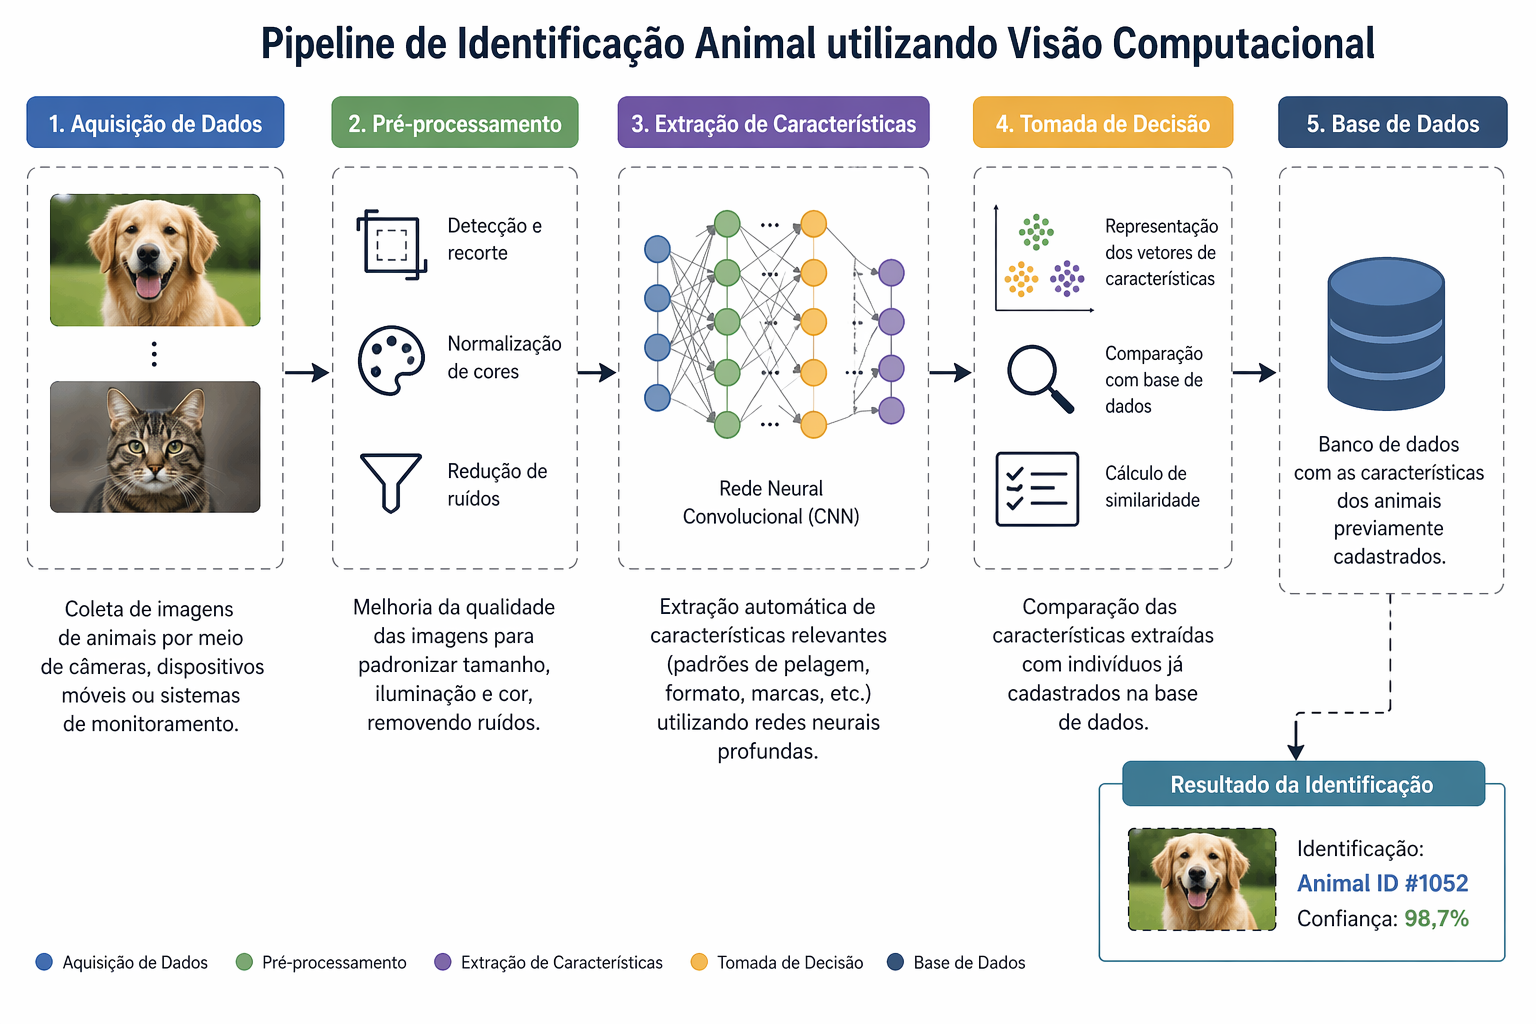
\includegraphics[scale=0.2]{Figs/identificacao.png}
\flushleft
\vspace{-0.2cm}
\hspace{0.9cm} \footnotesize Fonte: Elaborado pelo autor com base em \citeonline{vidal2021}.
\end{figure}

Conforme ilustrado na Figura \ref{fig:identificacao}, a identificação automatizada depende da combinação de diferentes etapas de processamento para transformar dados brutos em informações úteis. Inicialmente, os dados são coletados por meio de imagens ou sensores, sendo posteriormente tratados e analisados para extração de características relevantes. Essas informações são então utilizadas pelos algoritmos para reconhecer padrões e realizar a identificação do animal.

Esses sistemas representam uma das principais tendências tecnológicas relacionadas ao monitoramento e identificação animal, permitindo maior precisão na análise dos dados, automatização de processos e suporte à tomada de decisão em diferentes contextos da medicina veterinária e do cuidado animal \cite{vidal2021,arshad2025}.

\subsection{Tecnologias Aplicadas à Saúde Animal}

O crescimento da utilização de tecnologias digitais na medicina veterinária tem proporcionado avanços importantes relacionados ao gerenciamento da saúde animal. Sistemas digitais permitem registrar informações clínicas, organizar históricos médicos e facilitar o acompanhamento preventivo dos animais.

Segundo \citeonline{iskandar2023}, prontuários eletrônicos veterinários oferecem maior eficiência na gestão de dados clínicos, reduzindo erros humanos, melhorando a acessibilidade das informações e facilitando o acompanhamento médico. 

Os autores destacam que registros físicos apresentam limitações relacionadas à perda de dados, dificuldade de acesso e maior vulnerabilidade a falhas humanas. Nesse sentido, sistemas digitais tornam-se ferramentas importantes para modernização dos serviços veterinários e para a organização do histórico clínico dos animais.

Além disso, o acompanhamento preventivo possui papel fundamental na saúde animal. O controle de vacinação, por exemplo, permite prevenir doenças infecciosas e reduzir riscos relacionados à saúde pública. Sistemas digitais auxiliam nesse processo ao oferecer lembretes automáticos, armazenamento do histórico vacinal e acesso rápido às informações do animal \cite{MOUTINHO2017,iskandar2023}.

Outro ponto relevante refere-se à centralização das informações clínicas. Em muitos casos, dados relacionados ao animal encontram-se dispersos entre clínicas, documentos físicos e aplicações distintas, dificultando o acompanhamento contínuo da saúde do pet. A utilização de sistemas digitais contribui para reduzir essa fragmentação e facilitar o acesso às informações clínicas \cite{MORAES2024,iskandar2023}.

Dessa forma, soluções que integrem identificação animal, prontuário digital e acompanhamento vacinal tornam-se relevantes para otimizar os cuidados veterinários e melhorar a experiência dos tutores.

\subsection{Importância da Identificação para Controle e Segurança}

A identificação animal desempenha papel fundamental no controle sanitário, prevenção de doenças e segurança animal. Conforme destacado por \citeonline{murphy2008}, sistemas de rastreamento permitem respostas mais rápidas em situações de surtos epidemiológicos, facilitando o monitoramento e controle de doenças.

Além da saúde pública, esses sistemas também auxiliam na redução de abandono e perda de animais. Segundo \citeonline{sartori2018}, tecnologias de identificação aumentam significativamente as chances de recuperação de animais desaparecidos, além de fortalecer ações relacionadas à proteção animal.

Outro aspecto importante está relacionado às políticas públicas. O programa ProPatinhas, analisado por \citeonline{begnini2025}, demonstra como sistemas digitais podem auxiliar na construção de políticas voltadas ao bem-estar animal, registro populacional e controle de zoonoses. 

Além disso, estratégias de identificação e monitoramento são apontadas como mecanismos relevantes para fortalecimento das ações de proteção animal \cite{begnini2025,MOUTINHO2017}.

\subsection{Limitações das Tecnologias Atuais}

Apesar do avanço tecnológico observado nos últimos anos, muitas soluções ainda apresentam limitações importantes relacionadas à acessibilidade, integração e usabilidade. Diversos estudos apontam dificuldades relacionadas à dependência de dispositivos específicos, custos de implementação e fragmentação das informações clínicas e cadastrais dos animais \cite{zhao2020,sartori2018,MORAES2024}, entre os principais problemas identificados destacam-se:

\begin{itemize}
    \item Dependência de hardware específico, como leitores RFID e dispositivos NFC;
    
    \item Alto custo de implementação de soluções baseadas em inteligência artificial e análise genética;
    
    \item Falta de integração entre identificação, vacinação e histórico clínico;
    
    \item Complexidade técnica elevada para utilização cotidiana;
    
    \item Baixa acessibilidade para tutores sem conhecimento técnico;
    
    \item Dependência de conexão constante com internet em determinadas plataformas;
    
    \item Dificuldade de padronização e compartilhamento das informações entre diferentes sistemas.
\end{itemize}

Além disso, muitas aplicações disponíveis concentram-se apenas em funcionalidades específicas, como identificação, controle vacinal ou monitoramento veterinário, não oferecendo uma solução integrada para gerenciamento completo das informações relacionadas ao animal \cite{iskandar2023,MORAES2024}.

Dessa forma, evidencia-se a necessidade de sistemas mais acessíveis, centralizados e voltados à experiência prática do usuário.

\section{TRABALHOS CORRELATOS}

%% Remover comentario abaixo para o Projeto Inovador II
%\section{MATERIAIS E MÉTODOS}

O avanço das tecnologias digitais aplicadas ao cuidado com animais de estimação tem impulsionado o desenvolvimento de diferentes soluções voltadas à gestão de informações, monitoramento da saúde e identificação animal. Entretanto, embora esses sistemas apresentem contribuições relevantes, observa-se que muitos deles abordam o problema de forma fragmentada, concentrando-se em funcionalidades específicas.

No contexto da gestão clínica, Iskandar et al. \cite{iskandar2023} propõem um sistema eletrônico de prontuário médico animal voltado para ambientes veterinários. A solução tem como principal objetivo substituir registros físicos por um sistema digital estruturado, permitindo maior eficiência no gerenciamento de dados, acesso rápido às informações e redução de erros humanos. Além disso, o sistema busca auxiliar profissionais veterinários na organização do histórico clínico dos animais, tornando os processos mais rápidos e seguros.

A proposta apresenta uma abordagem robusta para uso profissional, sendo especialmente útil para clínicas e centros veterinários. Entretanto, sua utilização está centrada no ambiente institucional, não contemplando diretamente o uso cotidiano por tutores. Diferentemente deste trabalho, que busca oferecer praticidade e autonomia ao usuário comum, a proposta prioriza a administração clínica e o gerenciamento interno das informações.

De forma complementar, Vieira et al. \cite{vieira2025} apresentam uma plataforma web voltada ao gerenciamento de cuidados com animais e processos de adoção. O sistema integra funcionalidades como cadastro de pets, controle de vacinação, agendamento de consultas e interação entre usuários. A proposta destaca-se pela centralização de diferentes funcionalidades em um único ambiente, permitindo maior organização das informações e melhor acompanhamento dos cuidados relacionados aos animais.

Apesar da abrangência funcional, o sistema apresenta limitações relacionadas à experiência mobile, já que sua arquitetura é fortemente dependente do acesso via navegador web. Em comparação, o presente trabalho diferencia-se por priorizar mobilidade e acessibilidade multiplataforma, permitindo acesso rápido às informações em diferentes dispositivos e contextos de uso.

No que se refere à identificação animal, Sartori e Medeiros \cite{sartori2018} propõem uma solução baseada na tecnologia NFC (\textit{Near Field Communication}) para identificação de animais de estimação. O sistema permite armazenar informações do animal em dispositivos compatíveis, possibilitando acesso rápido aos dados por meio de leitura por aproximação.

A proposta apresenta caráter inovador ao utilizar tecnologias de comunicação por proximidade para auxiliar na identificação animal e na redução de casos de abandono. Contudo, sua utilização depende diretamente de dispositivos compatíveis com NFC, o que limita sua acessibilidade em larga escala. Além disso, o sistema concentra-se principalmente na identificação do animal, não contemplando funcionalidades mais amplas relacionadas ao acompanhamento de saúde e vacinação. Diferentemente dessa abordagem, o presente trabalho busca integrar a identificação e o gerenciamento de informações clínicas em um único ambiente digital acessível.

Sob uma perspectiva mais ampla e tecnológica, Arshad et al. \cite{arshad2025} exploram a aplicação de inteligência artificial no monitoramento da saúde e comportamento animal.

Os autores destacam que a utilização de inteligência artificial pode transformar significativamente os cuidados com animais de estimação, permitindo diagnósticos mais rápidos, monitoramento contínuo e análises preditivas. Além disso, o estudo apresenta exemplos de aplicações baseadas em dispositivos móveis, sensores inteligentes e sistemas automatizados de suporte veterinário.

Entretanto, apesar do elevado potencial tecnológico, tais soluções apresentam desafios relacionados ao alto custo de implementação, necessidade de infraestrutura avançada e complexidade computacional. Em contraste, o presente trabalho adota uma proposta mais acessível e prática, focada na resolução de problemas cotidianos relacionados ao gerenciamento de vacinação e identificação animal, sem depender de tecnologias avançadas ou equipamentos específicos.

Além disso, Begnini e Aguirre \cite{begnini2025} abordam a importância das políticas públicas voltadas à proteção e registro animal. O estudo destaca o programa ProPatinhas como iniciativa relevante para organização de dados, identificação e manejo ético de cães e gatos em âmbito nacional.

As autoras evidenciam que sistemas digitais podem contribuir significativamente para a construção de políticas públicas mais eficientes, auxiliando no controle populacional, na identificação e no acompanhamento animal. Contudo, a proposta possui foco institucional e governamental, direcionando-se à gestão pública e não ao uso individual por tutores.

Diferentemente dessa abordagem, o presente trabalho concentra-se na experiência cotidiana do usuário, oferecendo uma ferramenta digital voltada ao gerenciamento individual das informações do animal, com foco em praticidade, organização e acessibilidade.

Diante desses trabalhos, torna-se possível estabelecer uma comparação direta entre as soluções existentes e a proposta deste estudo, evidenciando diferenças importantes:

\begin{enumerate}[label=\alph*)]
    \item \textbf{Foco da aplicação:} enquanto sistemas como o de Iskandar et al. são voltados para clínicas veterinárias e o ProPatinhas para políticas públicas, o presente trabalho possui foco direto no tutor e no gerenciamento individual das informações do animal.

    \item \textbf{Escopo das funcionalidades:} o PetID concentra-se principalmente na identificação animal, enquanto o PetCare integra múltiplas funcionalidades relacionadas ao cuidado e adoção. Já a proposta deste trabalho busca integrar identificação e registro de vacinação de forma simplificada em um único ambiente digital.

    \item \textbf{Dependência tecnológica:} soluções como o PetID dependem de hardware específico (NFC), enquanto aplicações baseadas em inteligência artificial exigem infraestrutura computacional mais complexa. Em contraste, o sistema proposto busca acessibilidade e facilidade de utilização sem necessidade de tecnologias avançadas.

    \item \textbf{Mobilidade e acessibilidade:} sistemas web apresentam limitações em dispositivos móveis, enquanto a proposta deste trabalho prioriza acesso multiplataforma e disponibilidade das informações em diferentes contextos de uso.

    \item \textbf{Complexidade da solução:} abordagens baseadas em inteligência artificial apresentam maior complexidade técnica e custo de implementação. Já o presente trabalho adota uma solução mais leve, prática e voltada às necessidades cotidianas dos tutores.

    \item \textbf{Integração das informações:} grande parte dos trabalhos analisados aborda funcionalidades de maneira isolada, como identificação, gestão clínica ou monitoramento. Em contrapartida, este trabalho busca centralizar informações essenciais de saúde e identificação em um único sistema digital.
\end{enumerate}

Dessa forma, observa-se que os trabalhos analisados contribuem significativamente para o avanço das tecnologias voltadas ao cuidado animal. Entretanto, o presente estudo diferencia-se ao propor uma solução integrada, acessível e voltada ao uso cotidiano, priorizando praticidade, organização e facilidade de acesso às informações relacionadas aos animais de estimação.

\section{TRABALHO PROPOSTO}

Esta seção apresenta a solução que será desenvolvida neste trabalho, detalhando a proposta da aplicação, a arquitetura utilizada, a modelagem do banco de dados, as funcionalidades implementadas, as tecnologias empregadas durante o desenvolvimento e a metodologia adotada na construção do sistema.

O sistema, denominado \textbf{Registro Digital Animal}, será desenvolvido como uma aplicação multiplataforma baseada no conceito de \textit{Progressive Web App} (PWA), voltada para o gerenciamento digital de informações relacionadas à saúde e identificação de animais de estimação. A proposta surgiu a partir da necessidade de substituir registros físicos, como carteiras de vacinação e documentos veterinários, por um ambiente digital centralizado, acessível e de fácil utilização.

A aplicação permite que tutores realizem o cadastro de seus animais, armazenem informações vacinais, organizem documentos clínicos e acompanhem dados importantes relacionados ao cuidado animal. Além disso, o sistema também oferece funcionalidades complementares, como planejamento de viagens com pets, carteira digital e localização de clínicas veterinárias próximas.

Outro aspecto importante da proposta está relacionado à acessibilidade e mobilidade. Por ser desenvolvida como uma PWA, a aplicação pode ser utilizada diretamente pelo navegador, sem necessidade de instalação através de lojas de aplicativos, além de permitir funcionamento offline por meio de mecanismos de cache local.

\subsection{Arquitetura do Sistema}

A arquitetura da solução foi definida com o objetivo de garantir organização, desempenho e integração entre as diferentes funcionalidades do sistema. A aplicação adota o modelo cliente-servidor, permitindo separar a interface visual, o processamento das requisições e o armazenamento das informações.

Essa divisão facilita tanto a manutenção quanto a escalabilidade do sistema, além de permitir maior segurança e organização no gerenciamento dos dados relacionados aos animais e seus tutores.

A arquitetura do sistema é composta por três camadas principais:

\begin{itemize}
    \item \textbf{Frontend (PWA):} responsável pela interface visual da aplicação e pela interação com o usuário. O frontend será desenvolvido utilizando HTML5, CSS3 e JavaScript puro, funcionando como uma \textit{Progressive Web App}. Essa abordagem permite instalação em dispositivos móveis, funcionamento offline e melhor experiência de uso.

    \item \textbf{Backend (API REST):} responsável pelo processamento das requisições realizadas pela aplicação, autenticação de usuários, sincronização de informações e comunicação com o banco de dados. O backend foi implementado utilizando Node.js e arquitetura baseada em API REST.

    \item \textbf{Banco de Dados PostgreSQL:} responsável pelo armazenamento persistente das informações relacionadas aos usuários, animais, vacinas, documentos clínicos e demais dados utilizados pelo sistema.
\end{itemize}

A escolha dessa arquitetura ocorreu devido à necessidade de criar uma solução leve, organizada e acessível, permitindo que o sistema funcione de forma eficiente tanto em computadores quanto em dispositivos móveis.

Além disso, a separação em camadas facilita futuras expansões da aplicação, possibilitando implementação de novas funcionalidades sem comprometer a estrutura principal do sistema.

\subsection{Modelagem do Banco de Dados}

O banco de dados foi modelado com o objetivo de armazenar de forma organizada todas as informações relacionadas aos animais, seus tutores e registros clínicos. Para isso, foi utilizado o PostgreSQL, um sistema gerenciador de banco de dados relacional amplamente utilizado em aplicações web.

A modelagem contempla as principais entidades envolvidas no funcionamento do sistema, permitindo integração entre os diferentes módulos da aplicação.

\subsection{Funcionalidades Propostas}

O sistema a ser desenvolvido possuirá diferentes funcionalidades voltadas ao gerenciamento de informações relacionadas à saúde e identificação animal.

Entre as principais funcionalidades implementadas destacam-se:

\begin{enumerate}[label=\alph*)]
    \item \textbf{Cadastro e autenticação de usuários:} permite que tutores realizem cadastro e login na plataforma utilizando autenticação segura.

    \item \textbf{Cadastro de animais:} possibilita registrar informações completas dos pets, incluindo dados de identificação e observações clínicas.

    \item \textbf{Carteira digital do pet:} funcionalidade inspirada em documentos físicos tradicionais, permitindo acesso rápido às informações do animal.

    \item \textbf{Registro de vacinação:} permite armazenar o histórico vacinal do animal, incluindo controle de vencimento das vacinas.

    \item \textbf{Gerenciamento de documentos clínicos:} possibilita armazenar exames, receitas e documentos relacionados à saúde do animal.

    \item \textbf{Planejamento de viagens:} oferece checklist de itens importantes para transporte e viagens com pets.

    \item \textbf{Localização de clínicas veterinárias:} permite encontrar clínicas próximas ao usuário por meio de integração com mapas.

    \item \textbf{Funcionamento offline:} garante acesso às informações mesmo sem conexão com internet.

    \item \textbf{Instalação como PWA:} permite instalação da aplicação diretamente no dispositivo do usuário.

    \item \textbf{Tema claro e escuro:} possibilita personalização da interface conforme preferência do usuário.
\end{enumerate}

As funcionalidades serão desenvolvidas com foco na praticidade e organização das informações, buscando oferecer uma experiência simples e acessível aos tutores.

\subsection{Metodologia}

Esta pesquisa caracteriza-se como aplicada, pois busca desenvolver uma solução tecnológica voltada à resolução de um problema prático relacionado ao gerenciamento de informações de saúde animal.

Quanto à abordagem, a pesquisa possui caráter qualitativo, uma vez que o desenvolvimento da solução foi conduzido a partir da análise das necessidades dos usuários, funcionalidades implementadas e tecnologias utilizadas.

Em relação aos objetivos, a pesquisa pode ser classificada como exploratória e descritiva. Exploratória por investigar tecnologias e abordagens relacionadas à digitalização de registros veterinários e identificação animal. Descritiva por apresentar detalhadamente o desenvolvimento da aplicação e suas funcionalidades.

O método utilizado foi baseado em \textit{Design Science Research} (DSR), abordagem voltada à construção de artefatos tecnológicos capazes de solucionar problemas do mundo real.

O desenvolvimento do sistema ocorrerá nas seguintes etapas:

\begin{enumerate}
    \item Levantamento de requisitos;
    \item Definição da arquitetura do sistema;
    \item Modelagem do banco de dados;
    \item Desenvolvimento do backend;
    \item Desenvolvimento da interface frontend;
    \item Implementação das funcionalidades;
    \item Testes funcionais;
    \item Ajustes finais e documentação.
\end{enumerate}

\subsection{Recursos Necessários}

Para o desenvolvimento da aplicação, serão utilizados recursos de hardware e software.

Entre os principais recursos que serão utilizados, destacam-se:

\begin{itemize}
    \item Computador com sistema operacional Windows;
    \item Smartphone Android para testes da aplicação;
    \item Node.js para desenvolvimento do backend;
    \item PostgreSQL para gerenciamento do banco de dados;
    \item Visual Studio Code como ambiente de desenvolvimento;
    \item Navegadores Brave e Google Chrome para testes;
    \item GitHub para versionamento do projeto;
\end{itemize}

Todos os recursos utilizados no desenvolvimento são gratuitos ou possuem versões gratuitas disponíveis para utilização acadêmica.

\subsection{CRONOGRAMA}

O cronograma do projeto foi elaborado considerando todas as etapas necessárias para o desenvolvimento da aplicação, desde o levantamento inicial dos requisitos até a finalização da documentação do Trabalho de Conclusão de Curso. As atividades foram organizadas de maneira gradual, permitindo o desenvolvimento contínuo do sistema, realização de testes e refinamento das funcionalidades implementadas.

\renewcommand{\tablename}{Quadro}
\setcounter{table}{0}

\begin{table}[H]
\centering
\caption{Cronograma do projeto de pesquisa}
\vspace{-0.2cm}
\begin{tabular}{|p{8cm}|c|c|c|c|c|}
\hline
\multicolumn{6}{|c|}{\textbf{Cronograma de Trabalho de Conclusão de Curso}} \\
\hline
& \multicolumn{5}{|c|}{2º Semestre 2026} \\
\hline\hline
\textbf{Etapas} & Ago & Set & Out & Nov & Dez \\
\hline
Mapeamento dos requisitos e dados obrigatórios das cadernetas de vacinação & X & & & & \\
\hline
Modelagem do banco de dados e definição da arquitetura do sistema & X & X & & & \\
\hline
Desenvolvimento do backend (API REST, autenticação JWT, PostgreSQL) & X & X & X & & \\
\hline
Desenvolvimento do frontend (PWA, interface, Service Worker, offline) & & X & X & X & \\
\hline
Implementação da carteira digital, assinatura e exportação PDF & & & X & X & \\
\hline
Realização de testes funcionais em desktop e dispositivos móveis & & & X & X & \\
\hline
Redação do TCC Final & X & X & X & X & X \\
\hline
Elaboração da apresentação para defesa pública & & & & & X \\
\hline
\end{tabular}
\flushleft
\vspace{-0.1cm}
\hspace{0cm}\footnotesize Fonte: Elaborado pelo autor.
\end{table}

\section*{Declaração de Uso de Inteligência Artificial}
Os autores declaram que ferramentas de Inteligência Artificial generativa foram utilizadas exclusivamente como apoio auxiliar à elaboração deste trabalho, incluindo assistência na revisão linguística, estruturação textual e organização de ideias. Nenhuma ferramenta de IA foi utilizada para substituição da autoria intelectual, análise científica, interpretação dos resultados ou tomada de decisões acadêmicas. A responsabilidade integral pelo conteúdo, originalidade, veracidade das informações e conformidade com os princípios de integridade científica permanece integralmente atribuída aos autores.

\bibliographystyle{abntex2-unesc}
\renewcommand{\refname}{REFERÊNCIAS}
\bibliography{referencias} % arquivo referencias.bib que contém as referências bibliográficas utilizadas no artigo

%\setcounter{section}{}{} \label{app_a} % reset to start Attachment A
\renewcommand{\thesection}{APÊNDICE \Alph{section}}
\section{}
%São documentos elaborados pelo autor que servem como fundamentação (mapas, leis, estatutos). Deve ser precedido da palavra Apendice, identificada por letras maiúsculas consecutivas, travessão e pelo respectivo título. Utilizam-se letras maiúsculas dobradas quando esgotadas as letras do alfabeto. 



%\setcounter{section}{}{} \label{anex_a} % reset to start Attachment A
\renewcommand{\thesection}{Anexo \Alph{section}}
\section{}
%São documentos não elaborados pelo autor que servem como fundamentação (mapas, leis, estatutos). Deve ser precedido da palavra ANEXO, identificada por letras maiúsculas consecutivas, travessão e pelo respectivo título. Utilizam-se letras maiúsculas dobradas quando esgotadas as letras do alfabeto. 




\end{document} 

